\documentclass[11pt,twoside]{report}
\usepackage{preamble}
\graphicspath{{../img/cha1/}}
\setcounter{chapter}{1}
\renewcommand{\chaptername}{Appendix}
\renewcommand{\thechapter}{\Alph{chapter}}

\begin{document}

\chapter{Multi View Geometry}
\label{chapter:multi_view}

\epigraph{
A scientist \textbf{draws} what she \textbf{sees}
}{Barbara Lehn, \emph{What is a scientist}}

\section{Introduction}

This chapter include a very brief introduction to the key concepts about multi-view geometry. These ideals and equations are the corner stone, for implementing the algorithms (in appendix~\ref{chapter:algorithms}) introduced   in chapter~\ref{chapter:fish_3d}. More details on this subject is available in the celebrated text book by \citeauthor{hartley2003} \cite{hartley2003}.


\section{The Homogeneous Coordinates}


I will begin the introduction with the definition of homogeneous coordinates, where a normal Euclidian coordinate, say $(x, y)$ in $\mathbb{R}^2$, is uniquely represented as $(x, y, 1)$, which satisfies the following property
 
 $$
 (x, y, 1) = (kx, ky, k).
 $$
 
 \noindent This new vector with an extra ``1'' is called the homogeneous vector. The mapping from the Euclidian coordinates to their homogeneous counterparts is one-to-one and onto, and the \emph{inhomogeneous} representation of homogeneous vector $(x_1, x_2, x_3)$ is $(x_1/x_3, x_2/x_3)$. The projective transformation (to be introduced later) can be easily expressed as matrix multiplication of a $3 \times 3$ matrix and a $3 \times 1$ homogeneous vector, and this is the reason people slid an extra number into the homogeneous coordinates (represented by a homogeneous vector). Throughout this thesis, I will write the homogeneous representation of vector $\hat{\mathbf{x}} = (\mathbf{x}, 1)^T$ where $\mathbf{x}$ is the inhomogeneous representation of the vector\marginfootnote{The notation is different from the famous text book from \citeauthor{hartley2003} where the homogeneous coordinate is $\mathbf{x} = (\tilde{\mathbf{x}}, 1)^T$ and $\tilde{\mathbf{x}}$ represents the inhomogeneous representation\cite{hartley2003}. This eccentric option was selected, because most of the vectors in this thesis were inhomogeneous.}.
 
 The idea of expressing vectors as homogeneous coordinates is useful because the projective transformation can be expressed simply as a matrix production.
 
 \section{The Projective Transformation}
 
 \begin{SCfigure}
  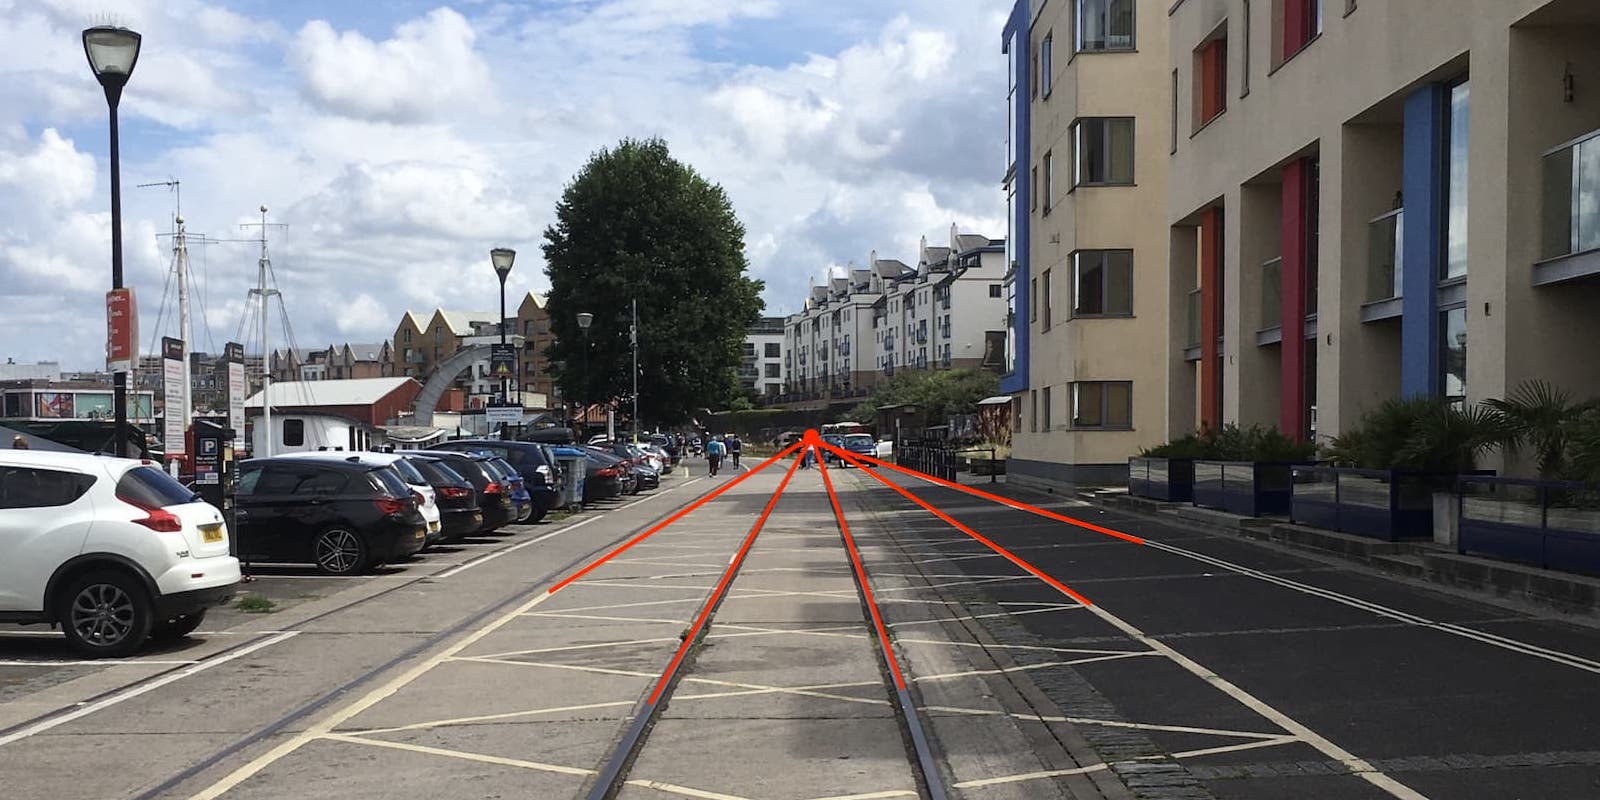
\includegraphics[width=\linewidth,outer]{ideal-point.jpg}
  \caption[An ideal point in Bristol harbourside]{A photo taken at the harbourside in Bristol, UK. The ideal point is labeled as the interception of parallel lines.}
  \label{fig:ideal-point}
\end{SCfigure}
 
The next concept to be introduced is the projection transformation, often represented by a \emph{homogeneous} matrix. For instance, a 2D projective transformation can be represented by matrix product, written as

$$
\hat{\mathbf{y}} = \mathbf{H} \hat{\mathbf{x}} = 
\left[
\begin{matrix}
	h_{11} & h_{12} & h_{13}\\
	h_{21} & h_{22} & h_{23}\\
	h_{31} & h_{32} & h_{33}\\
\end{matrix}
\right]
\left(
\begin{matrix}
	x_{1}\\ x_{2}\\ x_{3}\\
\end{matrix}
\right),
$$

\noindent where $\mathbf{H}$ is invariant by an overall rescaling, just like the homogeneous coordinates. A conceptually easy way to understand projection transformation, is to walk through the entire hierarchy of different transformations, from specific to general.
 
 \subsection{Euclidean Transformation}
 
 The Euclidean transformation, also known as the rigid transformation, is the most specific transformation. The 2D Euclidean transformation is composed of a rotation and a translation. The matrix representation of a such transformation is
 
$$
\begin{bmatrix}
	\cos\theta & -\sin\theta & t_{x}\\
	\sin\theta & \cos\theta & t_{x}\\
	0 & 0 & 1\\
\end{bmatrix} =
\begin{bmatrix}
	\mathbf{R} & \mathbf{t}\\
	\mathbf{0}^T & 1\\
\end{bmatrix},
$$

\noindent where $\mathbf{R} \in SO(2)$ is a rotation matrix, $\mathbf{t} \in \mathbb{R}^2$ is a vector, and $SO(2)$ is the 2D rotation group. As a rotation matrix, $\mathbf{R}$ has to satisfy the constrain that $\mathbf{R}\mathbf{R}^T = \mathbf{I}$. After the Euclidean transformation, a collection of points will have the same pairwise distances. 

\subsection{Similarity Transformation}

The similarity transformation is more general than its Euclidean counterpart, as it allows an extra overall scaling during the transformation. Specifically, the matrix representation of a 2D similarity is

$$
 \begin{bmatrix}
	s\mathbf{R} & \mathbf{t}\\
	\mathbf{0}^T & 1\\
\end{bmatrix},
$$

\noindent where $s$ controls the overall scaling. After the similarity transformation, a collection of points will have different pairwise distances, but the ratios of these distances remained unchanged.

\subsection{Affine Transformation}

The affine transformation, utilised widely in the study of driven systems, is a further generation of the similarity transformation. Typically, the matrix transformation of a 2D affinity is written as

$$
\begin{bmatrix}
	\mathbf{A} & \mathbf{t}\\
	\mathbf{0}^T & 1\\
\end{bmatrix},
$$

\noindent where $\mathbf{A} \in \mathbb{R}^{2 \times 2}$ is an arbitrary non-singluar matrix. It is more generalised because $\mathbf{A}$ does not have to be a rotation matrix. After the affine transformation, the parallel lines will remain being parallel.

\subsection{Projective Transformation as Generalised Affine Transformation}

The affine transformation is constrained by the fact that it will preserve the \emph{ideal point}. The ideal point is at infinity. A 2D ideal point can be written as $(\infty, \infty)^T$, whose homogeneous representation is $(x, y, 0)^T$. The affine transformation of such point is,

$$
\begin{bmatrix}
	\mathbf{A} & \mathbf{t}\\
	\mathbf{0}^T & 1\\
\end{bmatrix}
\begin{pmatrix}
	x \\ y \\ 0
\end{pmatrix}
=
\begin{pmatrix}
	\mathbf{A}
	\begin{pmatrix}
		x \\ y
	\end{pmatrix} \\
	0
\end{pmatrix}
= 
\begin{pmatrix}
	x\prime \\ y\prime \\ 0
\end{pmatrix}
$$

\noindent and the result $(x', y', 0)^T$ is still an ideal point, thanks to the $\mathbf{0}^T$ block in the matrix. Allowing the ideal point to move, we further generalised the affine transformation, and we get the projective transformation. The 2D projective transformation can be represented by the matrix

$$
\begin{bmatrix}
	\mathbf{A} & \mathbf{t}\\
	\mathbf{v}^T & \upsilon\\
\end{bmatrix}
$$

\noindent where $\mathbf{v} \in \mathbb{R}^2$ can take an value, and it is responsible for the movement of the ideal point. The value of $\upsilon$ is arbitrary, as the overall scaling of the matrix does not matter. The movement of the ideal point can be visualised by connecting parallel lines from a photo, as the parallel lines ``meet at the infinity point''. Figure \ref{fig:ideal-point} illustrates one ideal point from a photo taken by a mobile phone.


The important fact about projective transformation is that the collinearity is preserved. In other words, a straight line is still a straight line after the projective transformation.

\section{Representing Geometry Algebraically}


\begin{SCtable}
	\begin{minipage}[b]{\linewidth}
	\centering
	\begin{tabular}{ l c c }
		\toprule
		Name & Representation & Constrain\\
		\midrule
		2D Line & 
		$ \mathbf{l} = (a, b, c)^T$ &
		$\hat{\mathbf{x}}^T \mathbf{l} = 0$ \\
		2D Conic &
		\parbox{5cm}{
			$$
			\mathbf{C} =
			\begin{bmatrix}
			a & b/2 & d/2\\
			b/2 & c & e/2\\
			d/2 & e/2 & f
			\end{bmatrix}
			$$
		} &
		$ \hat{\mathbf{x}}^T \mathbf{C} \hat{\mathbf{x}} = 0$
		\\
		3D Quadric &
		\parbox{5cm}{
			$$
			\mathbf{Q} =
			\begin{bmatrix}
			a & b/2 & d/2 & e/2\\
			b/2 & e & f/2 & g/2\\
			c/2 & f/2 & h/2 & i/2\\
			d/2 & g/2 & i/2 & j\\
			\end{bmatrix}
			$$
		} &
		$ \hat{\mathbf{x}}^T \mathbf{Q} \hat{\mathbf{x}} = 0$
		\\
	\bottomrule
	\end{tabular}
	\end{minipage}
	
	\caption{Algebraic representation of different geometric entities.}
  \label{table:geometry}
\end{SCtable}


\section{The Camera Model}
\label{section:camera}

\begin{SCfigure}
  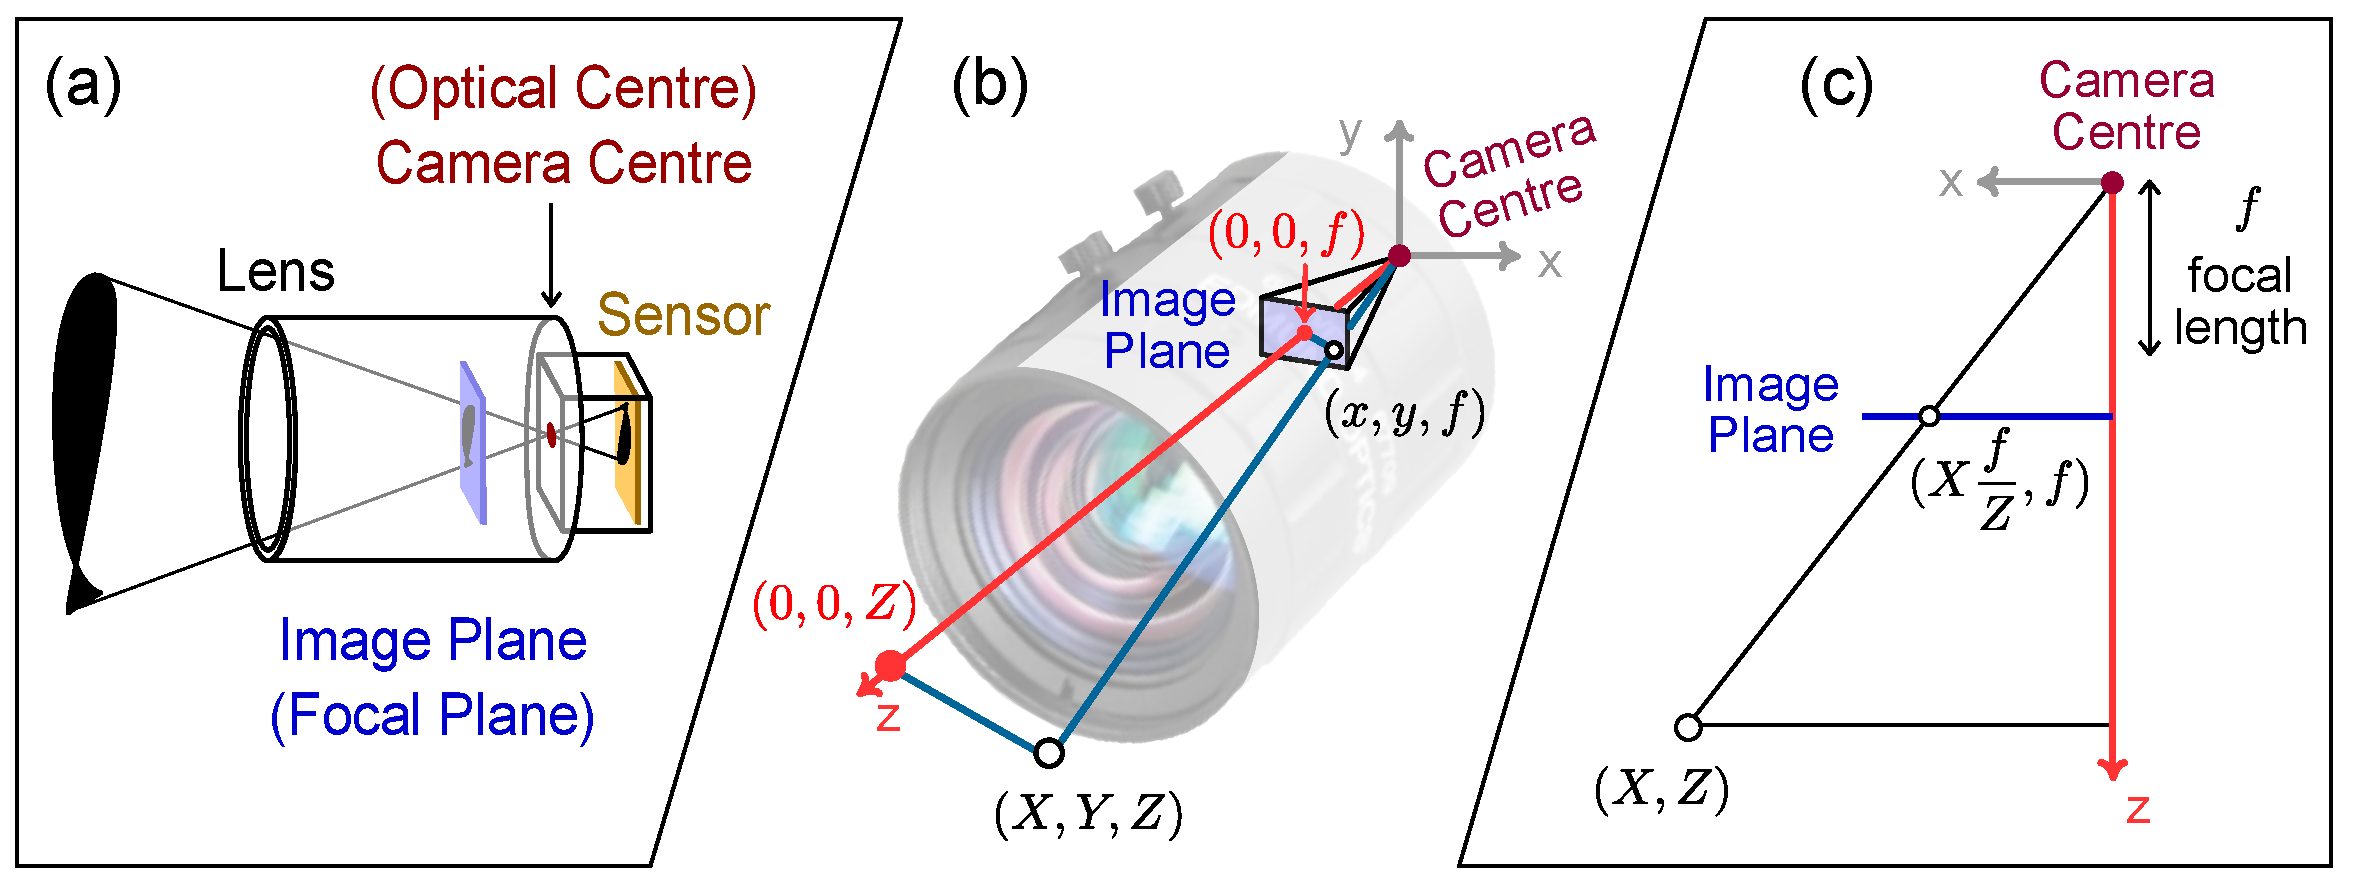
\includegraphics[width=\linewidth,outer]{camera-model}
  \caption[The pinhole camera model]{The pinhole camera model. (a) the projection transformation of the pinhole model, where the object projects virtually to the image plane and the camera sensor. (b) the coordination system centred defined by the image plane and camera centre. The point $(X, Y, Z)$ would be projected onto the image plane, with coordinates $(x, y, f)$.}
  \label{fig:camera_model}
\end{SCfigure}

In order to analyse the images taken by the camera, it is necessary to understand the projective transformations involved the photography. Most daily cameras can be effectively described by the pin--hole camera model, which is illustrated in Fig. \ref{fig:camera_model}. For a real object in 3D, its inverted image will be projected to the sensor in the camera, through the pin hole which is also known as the \emph{camera centre}. Then sensor then digitise the received signal and generate the image of the object.

\subsection{Single View Geometry}

Effectively, the inverted image on the sensor can be mapped to another virtual plane, the \emph{image plane}, who is in front of the camera centre. The 3D object casts an imaginary projection on the image plane, as shown in Fig.\ \ref{fig:camera_model}.

The camera centre and the image plane are the essential elements of the camera model, as they defined a (Cartesian) coordinate system, often referred to as the ``camera basis'' or ``camera frame''. For each camera, the origin of its basis is at its centre. The X and Y axes are defined by the image plane, and the Z axes is taken as the normal of the image plane. The camera frame is illustrated in Fig.\ \ref{fig:camera_model}.

The camera frame are often very different from the Cartesian coordinate system we use to describe the world. The two basis are related with

$$
\mathbf{X}_\text{cam} = \mathbf{R}(\mathbf{X} - \mathbf{C})
$$

\noindent where $\mathbf{X}_\text{cam}$ is the coordinate under the camera frame, and $\mathbf{X}$ is the coordinate under the world frame, for the same point. The matrix $\mathbf{R} \in SO(3)$ represents the relative orientation between the camera basis and the world basis, and the vector $\mathbf{C} \in \mathbb{R}^3$ is the location of the camera centre in the world frame.

Essentially, the formation of image can be described by 

$$
\hat{\mathbf{x}} = \mathbf{P} \hat{\mathbf{X}}
$$

\noindent where the matrix $\mathbf{P} \in \mathbb{R}^{3 \times 4}$ is called the projection matrix, the vector $\hat{\mathbf{X}} \in \mathbb{R}^4$ is the homogeneous representation of a 3D point. The 3D point will be projected on to the image, as a 2D point, whose homogeneous representation is $\hat{\mathbf{x}} \in \mathbb{R}^3$.

The projection matrix $\mathbf{P}$ encodes all the information about one camera, including the position, orientation, and other optical details. Such matrix can be decomposed into two parts, the intrinsic part and the extrinsic part, following

$$
\begin{aligned}
\mathbf{P}
&= \mathbf{K} [\mathbf{R}|\mathbf{t}] \\
&=
\underbrace{
	\begin{bmatrix}
		f_x & 0 & p_x \\
		0 & f_y & p_y \\
		0 & 0 & 1
	\end{bmatrix}
}_{\text{intrinsic}}
\underbrace{
	\left[
	\begin{array}{ccc|c}
		R_{11} & R_{12} & R_{13} & t_x\\
		R_{21} & R_{22} & R_{23} & t_y\\
		R_{31} & R_{32} & R_{33} & t_z
	\end{array}
	\right]
}_{\text{extrinsic}}.
\end{aligned}
$$

\noindent To understand these two parts, it is necessary to get familiar with 


\subsection{Two View Geometry}

A single object can be simultaneously captured by two cameras. And the same point in 3D, noted as $\mathbf{X} \in \mathbb{R}^3$, will have two different projections, $\mathbf{x}_1 \in \mathbb{R}^2$ and $\mathbf{x}_2 \in \mathbb{R}^2$, by camera 1 and 2 respectively. The homography $\mathbf{H}$ that transfer points on camera 1 to points on camera 2, is therefore constrained, because of the correspondence between $\mathbf{x}_1$ and $\mathbf{x}_2$ ($\mathbf{H}\hat{\mathbf{x}}_1 = \hat{\mathbf{x}}_2$). This epipolar geometry can be summarised algebraically by the fundamental matrix $\mathbf{F}$, which satisfies the constrain

$$
\hat{\mathbf{x}}_1  \mathbf{F}_{21}  \hat{\mathbf{x}}_2
= \mathbf{0}.
$$

Typically, the fundamental matrix yields two projection matrices in the \emph{canonical form}, written as

$$
\begin{aligned}
	\mathbf{P}_1 &= \left[\mathbf{I} | \mathbf{0}\right] \\
	\mathbf{P}_2 &= \left[ [\mathbf{e_2}]_\times \mathbf{F}_{12} | \mathbf{e_2} \right]
\end{aligned}
$$

\noindent where the $\mathbf{I} \in \mathbb{R}^{3\times3}$ is the identity matrix, $\mathbf{e}_2$ is the epipolar pole on camera 2, and $[\mathbf{a}]_\times$ yields the skew-symmetric matrix\marginfootnote{The cross product $\mathbf{a} \times \mathbf{b}$ can be expressed as $[\mathbf{a}]_\times \mathbf{b}$.} of vector $\mathbf{a} \in \mathbb{R}^3$. However, the mentioned camera pairs, $\mathbf{P}_1$ and $\mathbf{P}_2$, are not uniquely determined by their corresponding fundamental matrix. Given any projective transformation ($\mathbf{H} \in \mathbb{R}^{4 \times 4}$) , two pairs of camera matrices, $(\mathbf{P}_1, \mathbf{P}_2)$ and $(\mathbf{P}_1 \mathbf{H}, \mathbf{P}_2 \mathbf{H})$, share the same fundamental matrix. In other words, the fundamental matrix determines two camera matrices up to a projective ambiguity.

Given the intrinsic parameters of the two cameras, $\mathbf{K}_1$ and $\mathbf{K}_2$, one can calculate the \emph{essential matrix}, $$\mathbf{E} = \mathbf{K}_1^T \mathbf{F} \mathbf{K}_2$$, between two caneras. The essential matrix contains the information about the relative translation and rotation between the two cameras. It can be easily proved that the essential matrix is written as,

$$
\mathbf{E} = [\mathbf{t}]_\times \mathbf{R},
$$

\noindent where $\mathbf{t}$ is the translation between two cameras, and $\mathbf{R}$ is the rotation matrix that describes the relative orientation between the two cameras. The geometry of the rotation and translation operation is well summarised by the basis transformation

$$
\mathbf{X}_2 = \mathbf{R} \mathbf{X}_1 + \mathbf{t}
$$

\noindent where $\mathbf{X}_i$ is the coordinate of a 3D point relative to the coordinate system of camera $i$. The geometric between the basis, attached to the cameras, were illustrated in figure \ref{fig:camera_basis}.

\begin{SCfigure}
  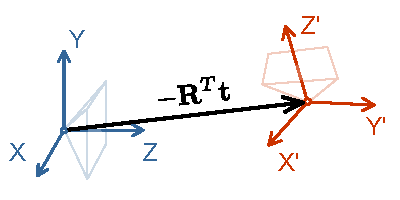
\includegraphics[width=0.6\linewidth,outer]{camera-basis-change}
  \caption[Relative orientation of cameras]{The relative orientation and translation between two cameras. The coordinate of the centre of camera 2, expressed in the basis attached to camera 1, is $-\mathbf{R}^T\mathbf{t}$. Notice the same point has the coordinate of $\mathbf{0}$ in the basis attached to camera 2.}
  \label{fig:camera_basis}
\end{SCfigure}

\subsection{Three View Geometry}

With the presence of three cameras, there are three fundamental matrices $\{\mathbf{F}_{21}, \mathbf{F}_{31}, \mathbf{F}_{32} \}$ corresponding to the three camera pairs. However, there is still another constrain on these fundamental matrices, written as \cite{hartley2003}

$$
\begin{aligned}
	  \hat{\mathbf{e}}_{23}^T\mathbf{F}_{21}\hat{\mathbf{e}}_{13}
	= \hat{\mathbf{e}}_{31}^T\mathbf{F}_{32}\hat{\mathbf{e}}_{21}
	= \hat{\mathbf{e}}_{32}^T\mathbf{F}_{31}\hat{\mathbf{e}}_{12}
	= 0
\end{aligned}
$$

\noindent where $\mathbf{e}_{ij}$ correspond to the epipolar pole of camera $j$ on the image captured by camera $i$; and $\mathbf{F}_{ij}$ satisfied the relation of $\mathbf{F}_{ij} \hat{\mathbf{x}}_j = \hat{\mathbf{l}}_i$ where $\mathbf{l}_i$ is the epipolar line on camera $i$. As a result, the geometric relationship between three cameras were described, algebraically, by the \emph{trifocal tensor}, written as

$$
\begin{aligned}
	\mathcal{T}_i^{jk} = a_i^j b_4^k - a_4^j b_i^k
\end{aligned}
$$

\noindent assuming the 3 cameras are in the canonical form, whose projection matrices are

$$
\mathbf{P}_1 = [\mathbf{I} | \mathbf{0}],
\mathbf{P}_2 = [a_j^i],
\mathbf{P}_3 = [b_j^i].
$$

The fundamental matrices can be recovered from the trifocal tensor, hence the relative poses between the cameras. The trifocal tensor can be used to calculate the extrinsic camera parameters.

\section{Camera Calibration}
\label{section:calibration}

In order to locate the fish in 3D, it is important to know the parameters of all the cameras. These parameters include the distortion coefficients and the projection matrices. From these matrices, the locations, orientations, and intrinsic parameters of the cameras can be obtained.

The workflow used in this thesis is as follows. Firstly I obtained the distortion coefficients and the intrinsic parameters of all the individual cameras. The task can be easily carried out with the \code{calibrateCamera} function in the ``opencv'' open--source project\marginfootnote{The opencv project was written in language C++ but provide a Python binding for all of its functions. I used the Python version in my code, with a slight different name: \texttt{calibrateCameraExtended}. Another popular option to carry out the same task would be the camera calibration tool box, cctb, written in MatLab language.}. This function use a non--linear optimisation, specifically the Levenberg-Marquardt algorithm, to optimise all the camera parameters, by minimising the reprojection error. Such error values were obtained by comparing the 2D feature points and the projected 3D objective points. Finally I calculate the extrinsic parameters, the positions and orientations, of all the cameras.

\begin{SCfigure}
  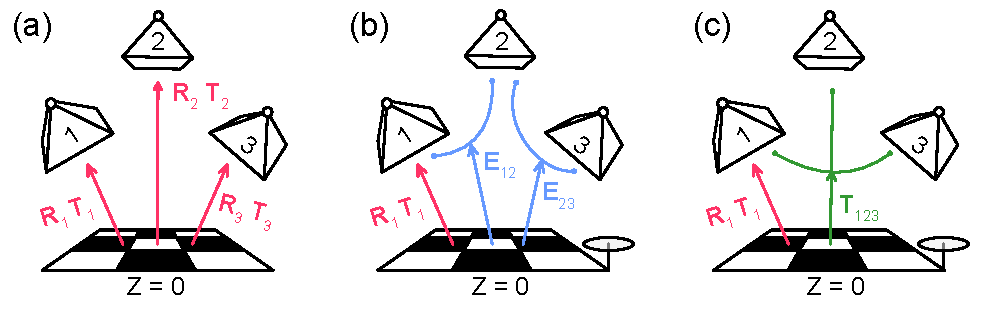
\includegraphics[width=1\linewidth,outer]{camera-calib-ext}
  \caption[Determining the extrinsic parameters of a camera]{Different ways to get the location ($\bf{T}$) and orientation ($\bf{R}$) of cameras using a chessboard. (a) The cameras obtain their individual $\bf{T}$ and $\bf{R}$ from the chessboard. (b) The chessboard offered the $\bf{T}$ and $\bf{R}$ of camera 1, as well as the essential matrices, $\bf{E}_{21}$ and $\bf{E}_{32}$. The relative translation and orientation of two cameras can be recovered from the essential matrices. (c) The chessboard offered the $\bf{T}$ and $\bf{R}$ of camera 1, as well as the trifocal tensor ($\bf{T}_{123}$). The tensor contain the information about the relative translation and orientation for all cameras.}
  \label{fig:calib-ext}
\end{SCfigure}

There are three possible ways to calculate the extrinsic parameters, with the help of a chessboard whose grid size is known. The methods were illustrated in Fig. \ref{fig:calib-ext}. The easiest one is to obtain the spatial information of the cameras from a chessboard, one--by--one, as shown in Fig. \ref{fig:calib-ext} (a). Specfically, the orientation and translation of the $i$th camera, represented by a rotational matrix $\mathbf{R}_i \in \mathrm{SO}(3)$ and a vector $\mathbf{T}_i \in \mathbb{R}^3$ respectively, can be found by minimising the reprojection error of the grid points on the chessboard. However, this plausible method is not ideal, because the obtained camera parameters, $\{\mathbf{R}_i\}$ and $\{\mathbf{T}_i\}$, are subjected to the errors of the 2D measurements (the locations of the corners on the chessboard are not perfect). As a result, the epipolar constrain on these cameras are violated, as the singular values of $\mathbf{E}_{ij}$ for camera $i$ and $j$. Such violation leads to mismatch between feature points.

A better approach would be calculate the camera matrices from the pairwise fundamental matrices. The fundamental matrix is the algebraic representation of the epipolar geometry between two cameras, containing the information about the relative translation and orientation between two cameras. 


In addition, the calibration board served as the anchor point, specifying the origin of the world coordinate system (the point of coordinate $(0, 0, 0)$). The $Z=0$ plane will be important in later sections, as a measure of the water level.


\section{Tutorial: Refining Calibration with Geometry}

The calibration method using the chessboard is convenient and easy. However, the practical results are not ideal. The overall performance of the calibration can be assessed by reconstructing the water--air interface in the image. The interface conics were highlighted in Fig.~\ref{fig:conic}, and these conics corresponds to a 3D circle at the plane where $Z=0$. The 3D circle can be reconstructed by the 2D conics, following the projective transformation

$$
\mathbf{Q} = \mathbf{P}^T \mathbf{C} \mathbf{P}
$$

\noindent where $\mathbf{Q} \in \mathbb{R}^4$ is the matrix representation of the quadric, and $\mathbf{C} \in \mathbb{R}^3$ is the matrix representing the conics. The point $\hat{\mathbf{X}} \in \mathbb{P}^3$ on the circle satisfies the constrains

$$
\begin{aligned}
\hat{\mathbf{X}}^T \mathbf{Q} \hat{\mathbf{X}} &= 0 \\
\hat{\mathbf{X}}^T \boldsymbol{\pi}_z &= 0,
\end{aligned}
$$

\noindent and $\boldsymbol{\pi}_z$ represents the $Z=0$ plane. The reconstructed circle can be represented by another conic, written as

$$
,
$$

\noindent and the coefficients can be transformed to the geometric coefficients: $x_c, y_c, a, b, \theta$, from which the conic is represented as,

$$
(x - xc)^2 / a + (y - yc)^2 / b = 0.
$$

The knowledge of the circle is not enough to uniquely determine the extrinsic parameters of one camera. Since 6 numbers (translation + rotation in 3D) are required to determine the camera pose, but one constrain is provided ($a = b$). For a three camera system, the conic will also provide 9 extra constrains, where

$$
\begin{aligned}
x_c^1 &= x_c^2 = x_c^3,\\
y_c^1 &= y_c^2 = y_c^3,\\
a^1 &= a^2 = a^3.
\end{aligned}
$$

\noindent and we can enforce these extra constrains during the camera calibration process, in order to improve the final estimation of the extrinsic parameter.

\begin{SCfigure}
  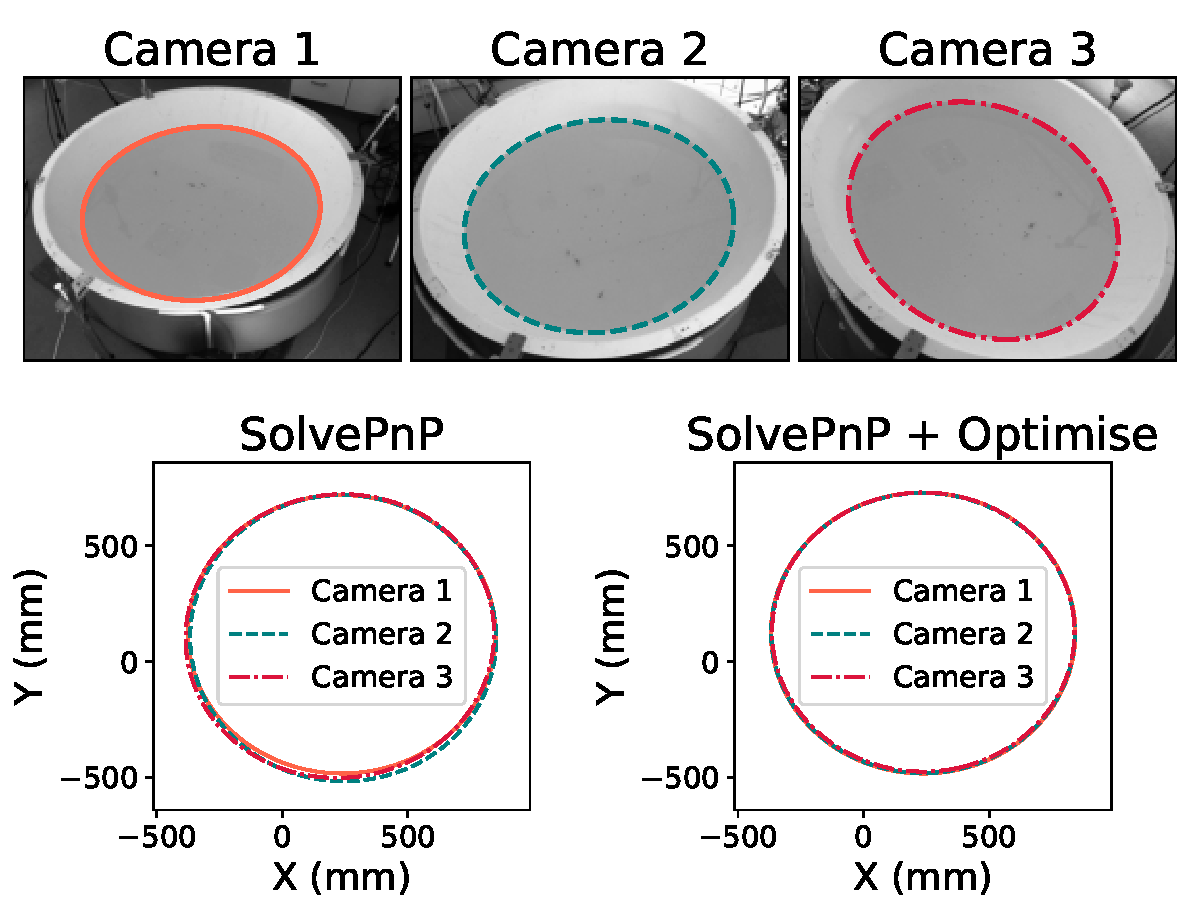
\includegraphics[width=1\linewidth,outer]{conic-3d}
  \caption[Conic optimisation for the camera calibration]{The conic features measured from the undistorted image. These feature points were fitted to get the conic matrices ($\mathbf{C}_{j}^{i}$ for the $j$th circle in camera $i$).}
  \label{fig:conic}
\end{SCfigure}




\end{document}
